\documentclass[tikz,border=10pt]{standalone}
\usepackage{tikz}
\usetikzlibrary{shapes.geometric,arrows.meta,positioning,fit,backgrounds,calc}

\begin{document}
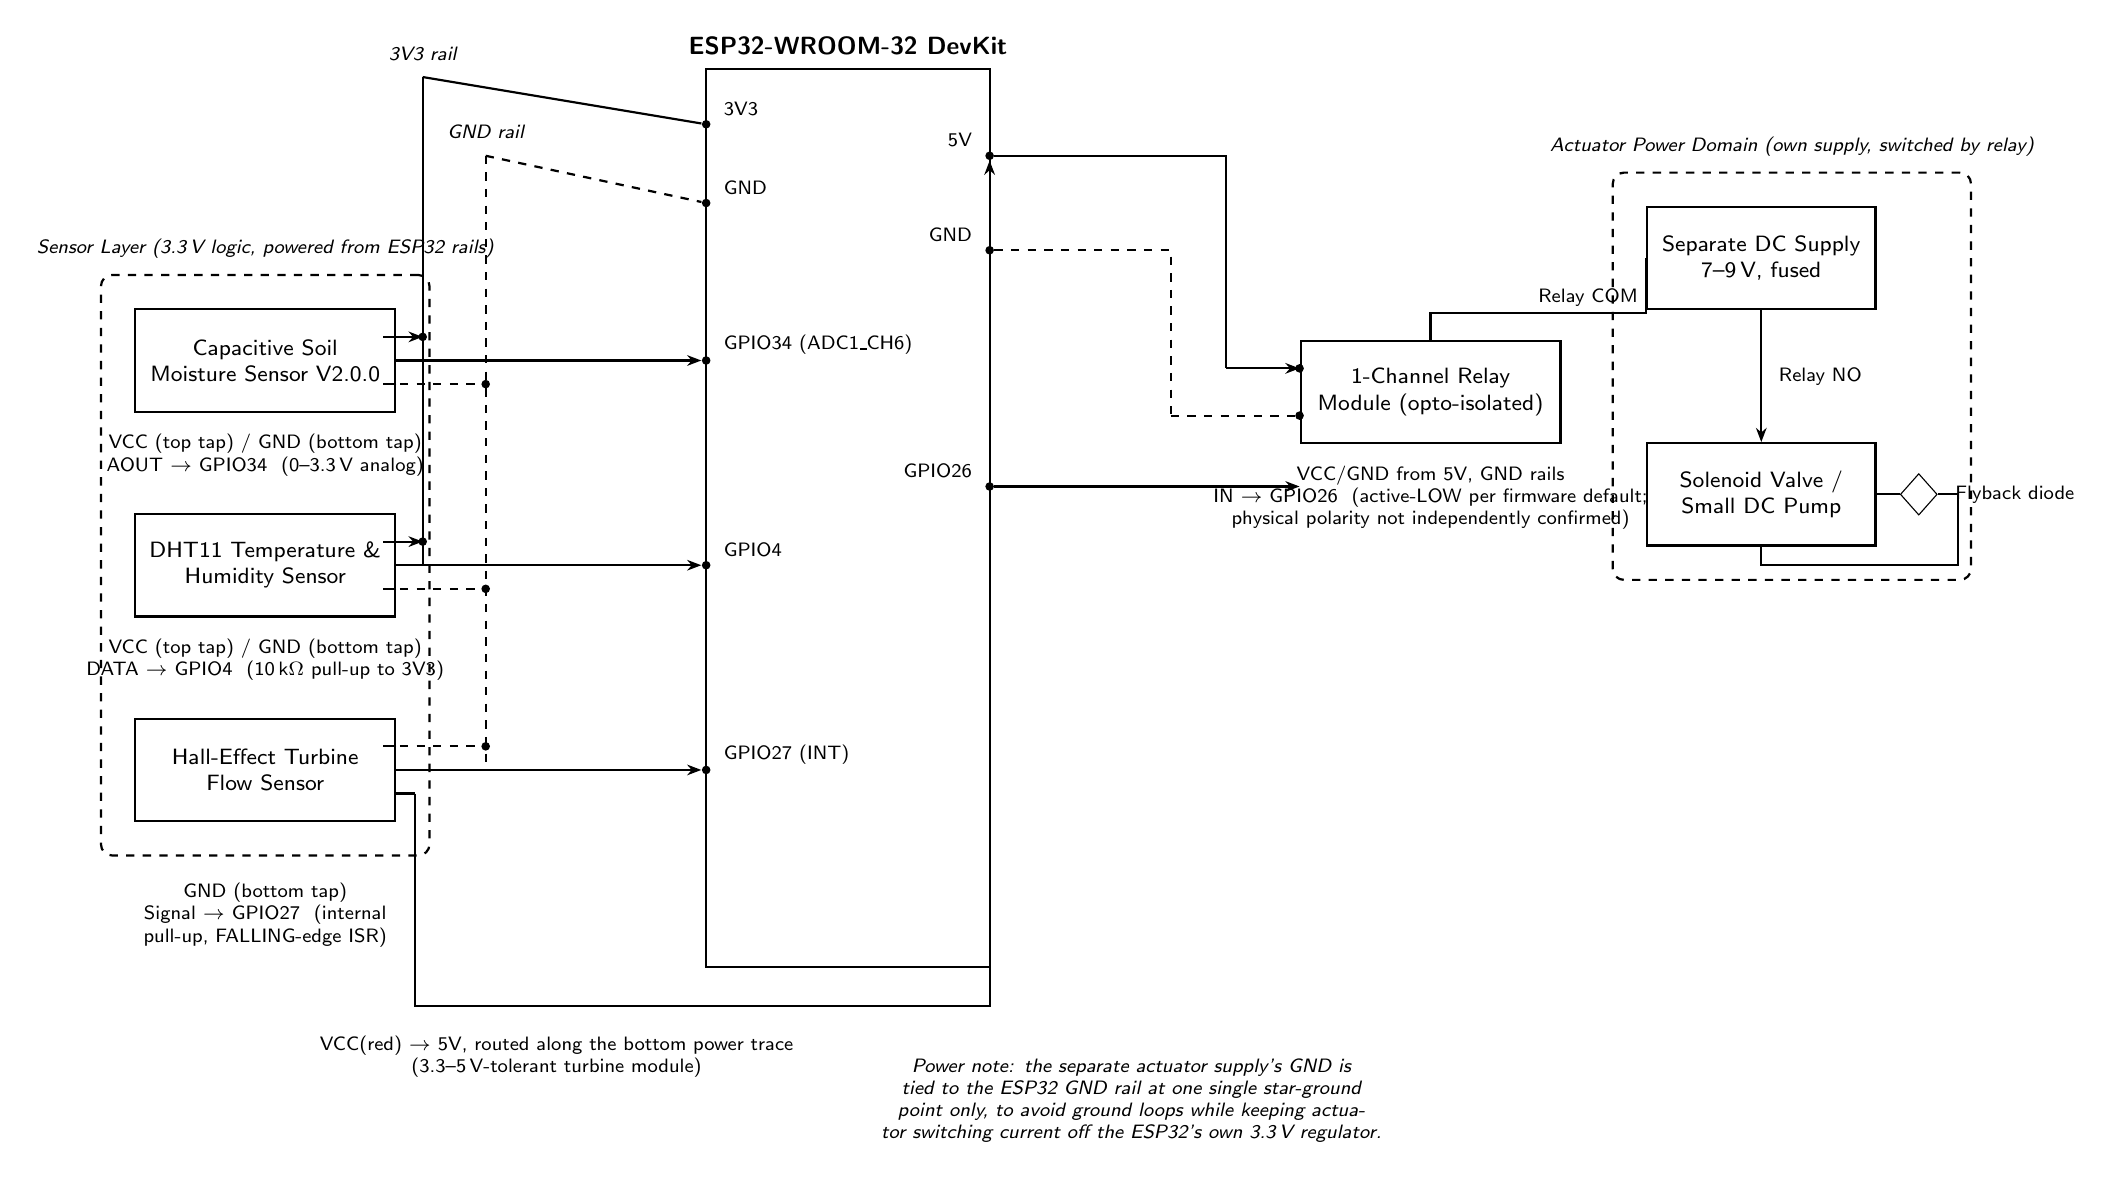
\begin{tikzpicture}[
  font=\sffamily\footnotesize,
  mcu/.style={draw, thick, rectangle, minimum width=3.6cm, minimum height=11.4cm, align=center, fill=white},
  dev/.style={draw, thick, rectangle, minimum width=3.3cm, minimum height=1.3cm, align=center, fill=white},
  pin/.style={font=\sffamily\scriptsize},
  raillbl/.style={font=\sffamily\scriptsize\itshape},
  wire/.style={thick},
  gndwire/.style={thick, dashed},
  arr/.style={-{Stealth[length=1.8mm]}, thick},
  junc/.style={circle, fill=black, inner sep=1.1pt}
]

% All coordinates are PLAIN (x,y) numbers in cm, chosen explicitly so every
% wire below is a single straight horizontal or vertical segment.

% ---- ESP32 body, centred at origin ----
\node[mcu] (esp) at (0,0) {};
\node[font=\sffamily\bfseries\small] at (0,6.0) {ESP32-WROOM-32 DevKit};

% ---- LEFT-edge pins (x = esp.west = -1.8) ----
\def\xL{-1.8}
\node[junc] (p3v3) at (\xL,5.0) {}; \node[pin, anchor=west] at (\xL+0.1,5.2) {3V3};
\node[junc] (pgndL) at (\xL,4.0) {}; \node[pin, anchor=west] at (\xL+0.1,4.2) {GND};
\node[junc] (p34)  at (\xL,2.0) {}; \node[pin, anchor=west] at (\xL+0.1,2.2) {GPIO34 (ADC1\_CH6)};
\node[junc] (p4)   at (\xL,-0.6) {}; \node[pin, anchor=west] at (\xL+0.1,-0.4) {GPIO4};
\node[junc] (p27)  at (\xL,-3.2) {}; \node[pin, anchor=west] at (\xL+0.1,-3.0) {GPIO27 (INT)};

% ---- RIGHT-edge pins (x = esp.east = 1.8) ----
\def\xR{1.8}
\node[junc] (p5v)  at (\xR,4.6) {}; \node[pin, anchor=east] at (\xR-0.1,4.8) {5V};
\node[junc] (pgndR) at (\xR,3.4) {}; \node[pin, anchor=east] at (\xR-0.1,3.6) {GND};
\node[junc] (p26)  at (\xR,0.4) {}; \node[pin, anchor=east] at (\xR-0.1,0.6) {GPIO26};

% =====================================================================
% LEFT SIDE: three sensors, each at the SAME y as its unique data pin
% =====================================================================
\node[dev] (soil) at (-7.4,2.0)  {Capacitive Soil\\Moisture Sensor V2.0.0};
\node[dev] (dht)  at (-7.4,-0.6) {DHT11 Temperature \&\\Humidity Sensor};
\node[dev] (flow) at (-7.4,-3.2) {Hall-Effect Turbine\\Flow Sensor};

% Bus rails: two vertical lines between sensors (x=-7.4) and MCU (x=-1.8)
\def\xVrail{-5.4}
\def\xGrail{-4.6}
\draw[wire]    (\xVrail,5.6) -- (\xVrail,-0.6);
\draw[wire]    (\xVrail,5.6) -- (p3v3);
\node[raillbl] at (\xVrail,5.9) {3V3 rail};

\draw[gndwire] (\xGrail,4.6) -- (\xGrail,-3.2);
\draw[gndwire] (\xGrail,4.6) -- (pgndL);
\node[raillbl] at (\xGrail,4.9) {GND rail};

% soil: VCC tap (upper stub), GND tap (lower stub), AOUT direct to GPIO34
\draw[wire,arr] (-5.9,2.3) -- (\xVrail,2.3) node[junc]{};
\draw[wire]     (soil.east |- 0,2.3) -- (-5.9,2.3);
\draw[gndwire]  (-5.9,1.7) -- (\xGrail,1.7) node[junc]{};
\draw[gndwire]  (soil.east |- 0,1.7) -- (-5.9,1.7);
\draw[wire,arr] (soil.east) -- (p34);
\node[pin, below=0.15cm of soil.south, align=center] {VCC (top tap) / GND (bottom tap)\\AOUT $\to$ GPIO34 \ (0--3.3\,V analog)};

% dht: VCC tap, GND tap, DATA direct to GPIO4
\draw[wire,arr] (-5.9,-0.3) -- (\xVrail,-0.3) node[junc]{};
\draw[wire]     (dht.east |- 0,-0.3) -- (-5.9,-0.3);
\draw[gndwire]  (-5.9,-0.9) -- (\xGrail,-0.9) node[junc]{};
\draw[gndwire]  (dht.east |- 0,-0.9) -- (-5.9,-0.9);
\draw[wire,arr] (dht.east) -- (p4);
\node[pin, below=0.15cm of dht.south, align=center] {VCC (top tap) / GND (bottom tap)\\DATA $\to$ GPIO4 \ (10\,k$\Omega$ pull-up to 3V3)};

% flow: GND tap to rail; Signal direct to GPIO27; VCC via bottom power trace to 5V
\draw[gndwire] (-5.9,-2.9) -- (\xGrail,-2.9) node[junc]{};
\draw[gndwire] (flow.east |- 0,-2.9) -- (-5.9,-2.9);
\draw[wire,arr] (flow.east) -- (p27);
\node[pin, below=0.65cm of flow.south, align=center, text width=3.3cm] {GND (bottom tap)\\Signal $\to$ GPIO27 \ (internal pull-up, FALLING-edge ISR)};

\draw[wire,arr] (-5.5,-3.5) -- (-5.5,-6.2) -- (\xR,-6.2) -- (p5v);
\draw[wire] (flow.east |- 0,-3.5) -- (-5.5,-3.5);
\node[pin, below=0.25cm of {(-3.7,-6.2)}, align=center] {VCC(red) $\to$ 5V, routed along the bottom power trace\\(3.3--5\,V-tolerant turbine module)};

% =====================================================================
% RIGHT SIDE: relay module and actuator power domain
% =====================================================================
\node[dev] (relay) at (7.4,1.6) {1-Channel Relay\\Module (opto-isolated)};

\def\xVrail2{4.8}
\def\xGrail2{4.1}
\draw[wire]    (p5v) -- (\xVrail2,4.6) -- (\xVrail2,1.9);
\draw[wire,arr] (\xVrail2,1.9) -- (relay.west |- 0,1.9) node[junc]{};
\draw[gndwire] (pgndR) -- (\xGrail2,3.4) -- (\xGrail2,1.3);
\draw[gndwire] (\xGrail2,1.3) -- (relay.west |- 0,1.3) node[junc]{};
\draw[wire,arr] (p26) -- (relay.west |- 0,0.4);
\node[pin, below=0.15cm of relay.south, align=center] {VCC/GND from 5V, GND rails\\IN $\to$ GPIO26 \ (active-LOW per firmware default;\\physical polarity not independently confirmed)};

\node[dev, minimum width=2.9cm] (psu) at (11.6,3.3) {Separate DC Supply\\7--9\,V, fused};
\node[dev, minimum width=2.9cm] (pump) at (11.6,0.3) {Solenoid Valve /\\Small DC Pump};

\draw[wire] (relay.north) -- (relay.north |- 0,2.6) -- (psu.west |- 0,2.6) -- (psu.west);
\node[pin] at (9.4,2.8) {Relay COM};
\draw[wire,arr] (psu.south) -- (pump.north);
\node[pin, right=0.1cm of {(11.6,1.8)}] {Relay NO};

\node[draw, diamond, minimum width=9pt, minimum height=15pt] (fd) at (13.6,0.3) {};
\draw[wire] (pump.east) -- (fd.west);
\draw[wire] (fd.east) -- (14.1,0.3) -- (14.1,-0.6) -- (11.6,-0.6) -- (pump.south);
\node[pin, right=0.1cm of fd] {Flyback diode};

% =====================================================================
% Power / grounding note
% =====================================================================
\node[pin, font=\sffamily\scriptsize\itshape, align=center, text width=8.0cm] at (3.6,-7.4)
  {Power note: the separate actuator supply's GND is tied to the ESP32 GND rail at one single star-ground point only, to avoid ground loops while keeping actuator switching current off the ESP32's own 3.3\,V regulator.};

\begin{scope}[on background layer]
\node[draw, dashed, thick, inner sep=12pt, rounded corners, fit=(soil)(dht)(flow)] (sensbox) {};
\node[font=\sffamily\scriptsize\itshape, above=2pt of sensbox.north] {Sensor Layer (3.3\,V logic, powered from ESP32 rails)};
\node[draw, dashed, thick, inner sep=12pt, rounded corners, fit=(psu)(pump)(fd)] (actbox) {};
\node[font=\sffamily\scriptsize\itshape, above=2pt of actbox.north] {Actuator Power Domain (own supply, switched by relay)};
\end{scope}

\end{tikzpicture}
\end{document}
